\documentclass[12pt]{article}

\usepackage[margin=0.8 in]{geometry}
\usepackage{amsmath}
\usepackage{amssymb}
\usepackage{macros}
\usepackage{mathtools}
\usepackage{enumerate}
\usepackage{verbatim}
\usepackage{amsthm}
\usepackage{hyperref}

\title{}
%\content{}



\let \proj \undefined
\renewcommand{\tr}{ \mathrm{tr}}
\DeclareMathOperator{\SU}{SU}
\DeclareMathOperator{\proj}{proj}
\newcommand{\sS}{\mathscr{S}}
\DeclareMathOperator{\comp}{comp}
\newcommand{\A}{\mathcal{A}}
\renewcommand{\D}{\mathcal{D}}
\renewcommand{\e}{\epsilon}
\newcommand{\et}{\tilde{\e}}
\newcommand{\vr}{\mathbf{r}}
\newcommand{\vF}{\mathbf{F}}
\newcommand{\triple}{\iiint_E f(x,y,z)dV}



\newenvironment{solution}
  {\begin{proof}[Solution]}
  {\end{proof}
  
  }
\newtheorem{example}{Example}
\newtheorem{exercise}{Exercise}
\newtheorem{theorem}{Theorem}
\newtheorem{definition}{Definition}
\renewcommand{\n}{\nabla}
\newcommand{\vu}{\vec{u}}
\newcommand{\gen}{(x_0,y_0,z_0)}
\newcommand{\bx}{\mathbf{x}}


\begin{document}
\section*{Directional Derivatives and the Gradient.}
What to know:
\begin{enumerate}
\item Be able to compute directional derivatives
\item Know the definition of the gradient, its two most important properties and be able to use them (not their proofs).
\end{enumerate}

In Calculus I, we saw that a derivative can be used to understand how a function changes near a given point. In Calculus 3, we talked about partial derivatives of a function $f(x,y)$, which capture a similar kind of information: how a function changes along two very specific directions, namely $x=const.$ and $y=const$. (if you want to think about it more geometrically, the partial derivatives capture the rate of change of the curves we find once we slice the graph of $f$ with planes parallel to the axes).

The question is, what if we'd like to see what happens in another direction? Is knowing just the partial derivatives at a point enough to determine what happens in other directions?

To answer this question, we introduce the directional derivative.

\begin{definition} If $\vu=\langle a,b\rangle$ is a \textbf{unit vector} and $f(x,y)$ is differentiable, then the directional derivative in the direction of $\vu$ is defined as $$D_{\vu} f(x_0,y_0)=\lim_{t\to 0}\dfrac{f(x_0+at,y_0+bt)-f(x_0,y_0)}{t}.$$
\end{definition}

As usual, this definition is not very useful for practical purposes. We can do a little computation and use the chain rule, to find that \begin{equation}\label{eq3}D_{\vu}f(x_0,y_0)=f_x(x_0,y_0)a+f_y(x_0,y_0)b=\langle f_x(x_0,y_0),f_y(x_0,y_0)\rangle \cdot\langle a,b\rangle.\end{equation} This is the formula we'll use in practice!

\textbf{Remark:} It is very important in the definition that the vector $\vu$ has unit length. If we are given a vector that is not of unit length and we are asked to find the directional derivative in the direction it determines, we have to turn it into a unit vector first by dividing it by its magnitude before we use it in the above formula.




\begin{example} Let $\theta\in[0,2\pi)$ be fixed. Then the unit vector that forms angle $\theta$ with the positive $x$ axis is $\vu=\langle\cos(\theta),\sin(\theta)\rangle.$ So if, for example $f(x,y)=3x^2+2yx+y^4$  and $\theta=\frac{\pi}{3}$, we have $$D_{\vu}f(x,y)=(6x+2y)\frac{1}{2}+(2x+4y^3)\frac{\sqrt{3}}{2}.$$
Evaluating at (1,2), we'd find
$$D_{\vu}(1,2)=5+17\sqrt{2}.$$
\end{example}
\subsection*{The Gradient}
From the formula in $\eqref{eq3}$, we see that the expression  $\langle f_x(x_0,y_0),f_y(x_0,y_0)\rangle$ includes all the information we need to determine the directional derivative in any direction at $x_0,y_0)$, so it's important enough to have a name. We define:
\begin{definition} If $f(x,y) $ is a differentiable function, its gradient at $(x_0,y_0)$ is defined to be the vector $$\n f(x_0,y_0)=\langle f_x(x_0,y_0),f_y(x_0,y_0)\rangle.$$
\end{definition}

An analogous definition holds in any dimension, for example:
\begin{definition} If $f(x,y,z) $ is a differentiable function, its gradient at $(x_0,y_0,z_0)$ is defined to be the vector $$\n f(x_0,y_0,z_0)=\langle f_x(x_0,y_0,z_0),f_y(x_0,y_0,z_0),f_z(x_0,y_0,z_0)\rangle.$$
\end{definition}
\textbf{Remark:} Other notations for the gradient include $\grad f$ and $df$.

We will now see two properties of the gradient that make it a really important object. They are stated in three dimensions, but they hold unchanged in any dimension.

\subsection*{The gradient gives the direction of maximum net rate of change}
The first reason why the gradient is important is the following theorem, which says that the $\n f$ points to the direction where $f$ increases the fastest, whereas $-\n f$ points towards the direction in which $f$ decreases the fastest :
\begin{theorem} Let $f(x,y,z)$ be a differentiable function, and suppose that $\n f(x_0,y_0,z_0)\neq 0$. Then for any unit vector $\vu$ we have $$D_{-\frac{\n f(x_0,y_0,z_0)}{|\n f(x_0,y_0,z_0)|}}f(x_0,y_0,z_0)\leq D_{\vu}f(x_0,y_0,z_0)\leq D_{\frac{\n f(x_0,y_0,z_0)}{|\n f(x_0,y_0,z_0)|}}f(x_0,y_0,z_0).$$ Moreover, the maximum net rate of change at $\gen$ is $|\n f(x_0,y_0,z_0)|$ and the minimum net rate of change is $-|\n f(x_0,y_0,z_0)|$.
\end{theorem}
\begin{proof} Take any unit vector $\vu$. Then \begin{align*}
D_{\vu}f=\n f\cdot \vu=|\n f||\vu|\cos(\theta)=|\n f|\cos(\theta),
\end{align*}
where $\theta$ is the angle between $\n f\gen$ and $\vu$, and we also used that $\vu$ is a unit vector. Since $-1\leq \cos(\theta)\leq 1$, we find
\begin{align}
-|\n f| \leq |\n f|\cos(\theta)\leq |\n f|,
\end{align} or
\begin{equation}
\label{eq2} -|\n f| \leq D_{\vu}f\leq |\n f|.
\end{equation}

However, $$D_{\frac{\n f}{|\n f|}}f=\frac{\n f}{|\n f|}\cdot\n f=\frac{|\n f|^2}{|\n f|}=|\n f|,$$ and $$D_{-\frac{\n f}{|\n f|}}f=-\frac{\n f}{|\n f|}\cdot\n f=-\frac{|\n f|^2}{|\n f|}=-|\n f|,$$
Together with \eqref{eq2}, we find  $$D_{-\frac{\n f}{|\n f|}}f\leq D_{\vu}f\leq D_{\frac{\n f}{|\n f|}}f$$ and this shows the theorem.
\end{proof}


\begin{example} Find the maximum rate of change of $f(x,y)=x^2y+yx$ at $(1,2)$ and the direction in which it happens.
\end{example}
\begin{solution} We find the gradient: $$\n f(1,2)=\langle 2xy+y,x^2+x\rangle_{|(1,2)}=\langle 6,2 \rangle.$$

This tells us that the maximum rate of change is $$D_{\vu} f=2\sqrt{10}.$$ in the direction determined by $\langle 6,2 \rangle$.
\end{solution}

\begin{example} The Gradient Descent Algorithm: a widely used iterative algorithm to find local minima of a function $f$ of many variables. It starts with some initial $\bx^{(0)}$ and performs the iteration $$\bx^{(n+1)}=\bx^{(n)}-\alpha \n f(\bx^{(n)}),$$ where $\alpha $ is a fixed parameter (in some versions of the algorithm you can allow it to change at each step). Can you explain why such an algorithm would lead us towards a local minimum?
\end{example}

\begin{figure}
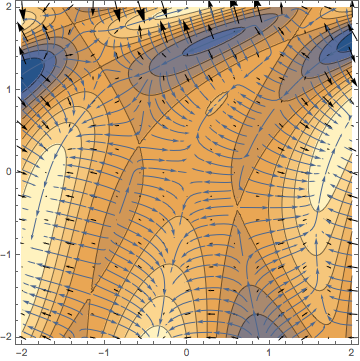
\includegraphics[scale=.5]{graphic.png}
\caption{The level curves of a function, plotted together with its gradient at each point. Warm colors correspond to large values, cold colors correspond to small values.}
\end{figure}

\subsection*{The gradient is orthogonal to the level curves/surfaces.}
The second reason why the gradient is a very important object is the following theorem:
\begin{theorem}
If $f(x,y,z)$ is a differentiable function then the gradient $\nabla f (x_0,y_0,z_0)$ is orthogonal to the tangent plane to the level surface of $f$ at $(x_0,y_0,z_0)$.
\end{theorem}
\begin{proof}
We will show that the gradient is perpendicular to the initial velocity of every curve $\g (t)=(x(t),y(t),z(t))$ in the level surface through $(x_0,y_0,z_0)$ that starts at $(x_0,y_0,z_0)$. Suppose that $f(x_0,y_0,z_0)=c$, so that the level set through $( x_0,y_0,z_0)$ is $$S=\{(x,y,z):f(x,y,z)=c\}.$$

Then $f(\g(t))=c$ for all $t$ because we assumed that it is a curve inside the level set $S$, and $\g(0)=(x_0,y_0,z_0)$. Therefore, \begin{align*}
\frac{d}{dt}(f(\g(t))_{|t=0}=0&\implies (\frac{\p f}{\p x}\frac{\p x}{\p t}+\frac{\p f}{\p y}\frac{\p y}{\p t}+\frac{\p f}{\p z}\frac{\p z}{\p t})_{|t=0}=0\\
&\implies \nabla f(\g(0))\cdot \g'(0)=0.
\end{align*}
This is saying that $\nabla f(x_0,y_0,z_0)$ is perpendicular to $\g'(0)$, and $\g$ was arbitrary. This shows that $\nabla f(x_0,y_0,z_0)$ is orthogonal to the level set $S$ at $(x_0,y_0,z_0)$.
\end{proof}


\subsubsection*{Tangent planes}
We can use this property of the gradient to compute tangent planes of level sets easily. Recall from Math 126 that given a point $p=(x_0,y_0,z_0)$ and a vector $v=(a,b,c)$, the plane through $p$ with normal vector $v$ was given by $$a(x-x_0)+b(y-y_0)+c(z-z_0)=0.$$

So, the tangent plane of a level set $$S=\{(x,y,z):F(x,y,z)=c\}$$ at $\gen$ is given by $$\p_xF (x_0,y_0,z_0)(x-x_0)+\p_yF(x_0,y_0,z_0)(y-y_0)+\p_z F(x_0,y_0,z_0)(z-z_0)=0$$ or \begin{equation}\label{eq1}\nabla F(x_0,y_0,z_0)\cdot\langle x-x_0,y-y_0,z-z_0\rangle=0.\end{equation}
\begin{exercise} Use \eqref{eq1} to find the level set of the function $F(x,y,z)=y^2z^3+3zy+2xz+2$ at $(-6,2,1)$. Compare your answer to the last example of the previous section.
\end{exercise}
\end{document}

